\documentclass[12pt,b5paper]{ltjsarticle}

%\usepackage[margin=15truemm, top=5truemm, bottom=5truemm]{geometry}
\usepackage[margin=15truemm]{geometry}

\usepackage{amsmath,amssymb}
%\pagestyle{headings}
\pagestyle{empty}

%\usepackage{listings,url}
\renewcommand{\theenumi}{(\arabic{enumi})}

\usepackage{graphicx}

\usepackage{tikz}
\usetikzlibrary {arrows.meta}
\usepackage{wrapfig}	% required for `\wrapfigure' (yatex added)
\begin{document}

 \begin{equation}
  a = \sum_{n=0}^{\infty} a_n (x-a)^n
 \end{equation}


\hrulefill

関数の収束はいくつかあり、それぞれで意味がある。

関数$f(x)$の定義域$D$とする。
\begin{enumerate}
 \item ある点$p\in D$で関数$f(x)$が収束
       \label{094401_31Mar22}
 \item 定義域$D$において関数$f(x)$が各点収束
       \label{094522_31Mar22}
 \item 定義域$D$において関数$f(x)$が一様収束
       \label{094641_31Mar22}
\end{enumerate}

\dotfill

\ref{094401_31Mar22} は 数列の無限和(級数)が値を持つことと同じ。

\ref{094522_31Mar22} は 定義域$D$ の任意の点において
%\ref{094401_31Mar22} のように
収束する。
これは全ての点を取り出して一点ずつ収束することで、
$p\in D$ごとの収束する速さは問わない。

\ref{094641_31Mar22} は 定義域$D$ の点に依存せず
$D$上で収束する。
これは各点の収束する速さが一定で抑えられるので
それぞれの点で同じような速さ(一様)で収束する。

\hrulefill

 \begin{equation}
  a_0 =
   \begin{cases}
    \sup A \quad ( | \sup A -a | \geq | \inf A -a |)\\
    \inf A \quad ( | \sup A -a | < | \inf A -a |)\\
   \end{cases}
 \end{equation}

$a_0$を定義域の端の値($\sup A$又は$\inf A$)を利用するのは
問題の式の $a$ からより遠い値を選ぶことで
収束しづらい状況を考えているのではないか。

定義域$A$が $[-a_0, a_0]$(又は$[a_0, -a_0]$)の部分集合となるので
$[-a_0, a_0]$(又は$[a_0, -a_0]$)で一様収束するなら
 $A$ でも一様収束するということを示したいのではないかと思う。


\newpage

定義域$A$(閉集合)上の関数$f(x)$について
 \begin{equation}
  f(x) = \sum_{n=0}^{\infty} a_n (x-a)^n
 \end{equation}

先頭の項$a_0$を次のように置く。
 \begin{equation}
  a_0 =
   \begin{cases}
    \sup A \quad ( | \sup A -a | \geq | \inf A -a |)\\
    \inf A \quad ( | \sup A -a | < | \inf A -a |)
   \end{cases}
 \end{equation}

これは$f(x)$の中心$a$から定義域の遠い方の値を$a_0$としている。

$a$が$A$の中央より小さいと次のような配置になる。

\begin{tikzpicture}
  \draw (0,0)--(10,0);
%  \foreach \x in {-5,...,5} \draw (\x,0)--(\x,-0.2) node[below] { $\x$ };
 \draw (5,0)--(5,-0.1) node[below]{$a$};
 \draw (4,0)--(4,0.2);
 \draw (7,0)--(7,0.2);
 \draw (4,0.2)--(7,0.2);
 \draw (5.5, 0.2) node[above]{$A$};
 \draw (7,0)--(7, -0.1) node[below]{$a_0$};
 \draw (3, -1)--(7, -1);
 \foreach \x in {3, 5, 7} \draw (\x,-0.9)--(\x,-1.1);
 \foreach \x in {4, 6} \draw (\x,-1.2) node[below]{$a_0-a$};
 \draw (3,0)--(3, -0.1) node[below]{$2a-a_0$};
\end{tikzpicture}

これにより 閉区間$[2a-a_0, a_0]$ は
$A\subset [2a-a_0, a_0]$ となる。

逆に$a$が中央より大きいと
$A\subset [a_0, 2a-a_0]$ となる。


\newpage

定理

関数$f(x)$の収束半径を$r$とする。
 \begin{equation}
  f(x) = \sum_{n=0}^{\infty} a_n (x-a)^n
 \end{equation}

$r>0$ のとき、
空でない閉集合$A\subset \mathbb{R}$を
$A\subset (a-r,\,a+r)$となるように任意に選んでおく。
このとき、$f(x)$は$A$を定義域として考えると
一様収束する。

$r=+\infty$の場合、$A$を$\mathbb{R}$の有界な閉集合とすると一様収束する。

\hrulefill

関数$f(x)$は次のような式である。
 \begin{equation}
  f(x) =% \sum_{n=0}^{\infty} a_n (x-a)^n
   a_0 + a_1(x-a) + a_2(x-a)^2 + a_3(x-a)^3 + a_4(x-a)^4 + \cdots
 \end{equation}
この式の係数$a_n$は収束半径などとは無関係に先に決定されている。
しかし、$a_0$は$f(x)$の定数項であり、収束性に関係しない。
例えば、この式の両辺から$a_0$を引いた式
 \begin{equation}
  f(x) - a_0 =% \sum_{n=0}^{\infty} a_n (x-a)^n
   a_1(x-a) + a_2(x-a)^2 + a_3(x-a)^3 + a_4(x-a)^4 + \cdots
 \end{equation}
は収束値が$f(x)$とは異なるが、収束の仕方は同じである。
そこで、次のように置きなおす。
 \begin{equation}
  a_0 =
   \begin{cases}
    \sup A \quad ( | \sup A -a | \geq | \inf A -a |)\\
    \inf A \quad ( | \sup A -a | < | \inf A -a |)
   \end{cases}
 \end{equation}

これにより$a_0$は閉集合$A$の端点となり、$a_0\in A$となる。
位置関係は次の図の場合か左右を反転させた図になる。

\begin{tikzpicture}
  \draw [->] (0,0)--(10,0);
%  \foreach \x in {-5,...,5} \draw (\x,0)--(\x,-0.2) node[below] { $\x$ };
 \draw (5,0)--(5,-0.1) node[below]{$a$};
 \draw (4,0)--(4,0.2);
 \draw (7,0)--(7,0.2);
 \draw (4,0.2)--(7,0.2);
 \draw (5.5, 0.2) node[above]{$A$};
 \draw (7,0)--(7, -0.1) node[below]{$a_0$};
% \draw (1, -1)--(9, -1);
% \foreach \x in {1, 5, 9} \draw (\x,-0.9)--(\x,-1.1);
% \foreach \x in {3, 7} \draw (\x,-1.2) node[below]{$r$};
% \draw (3,0)--(3, -0.1) node[below]{$2a-a_0$};
 \draw (1,0)--(1, -0.1) node[below]{$a-r$};
 \draw (9,0)--(9, -0.1) node[below]{$a+r$};
\end{tikzpicture}

 \begin{tikzpicture}
  \draw [->] (0,0)--(10,0);
  \draw (5,0)--(5,-0.1) node[below]{$a$};
  \foreach \x in {6, 8} \draw (\x,0)--(\x,0.2);
  \draw (6,0.2)--(8,0.2);
  \draw (7, 0.2) node[above]{$A$};
  \draw (8,0)--(8, -0.1) node[below]{$a_0$};
  \draw (1,0)--(1, -0.1) node[below]{$a-r$};
  \draw (9,0)--(9, -0.1) node[below]{$a+r$};
 \end{tikzpicture}

点$a, a_0$や閉集合$A$は収束円$(a-r,a+r)$に必ず含まれるが、
集合$A$に点$a$が含まれるかどうかは$A$のとり方による。

$a_0$を上記のようにおいたことで、
$a=a_0$の時は一点だけの集合$A=\{a\}$となり、
$a\ne a_0$の時は $| a_0 -a | < r$であり、
${}^\forall x\in A$に対し$x\leq a_0$(又は$x\geq a_0$)となり
証明するのに都合が良い。



\newpage


\begin{equation}
 f_n(x)=x^n \qquad g_n(x)=(x-6)^n
\end{equation}

\begin{wrapfigure}{r}{200pt}%{0.45\textwidth}
 \begin{center}
  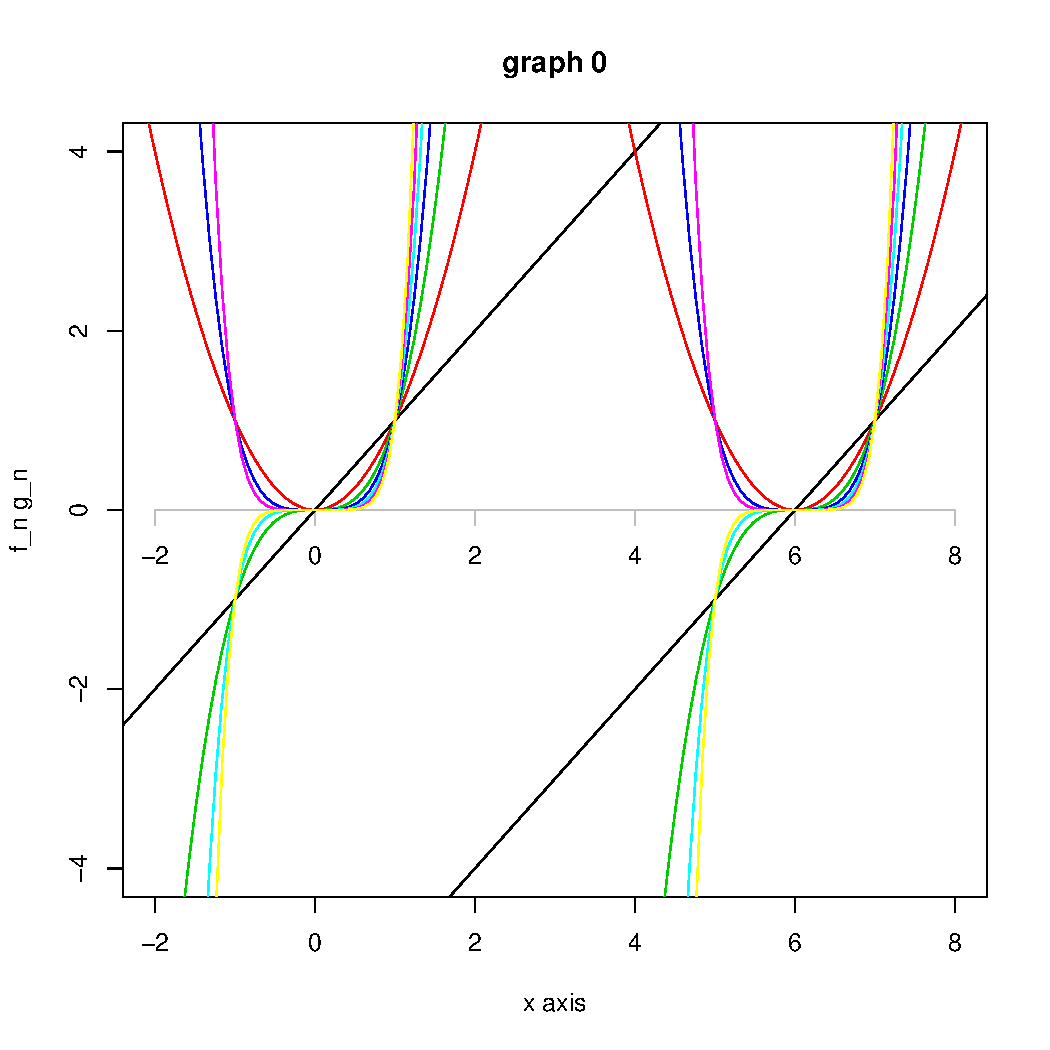
\includegraphics[scale=0.4]{graph1_R.pdf}
 \end{center}
\end{wrapfigure}
関数$f_n$は収束半径$r=1$の関数です。
区間$(-1,1)$において$\lim_{n\rightarrow\infty} f_n(x)=0$です。
関数$g_n$は$f_n$を横に$6$ずらした関数です。
ずれた分が式に現れていますが、これが収束円の中心となっています。
収束半径は$f_n$と同じです。
区間$(5,7)$で収束します。
図は$n=1,\dots,7$の時の$f_n$と$g_n$です。

%\vspace{100pt}

\quad

\quad

\quad

\begin{equation}
 \hat{f}_n(x)=a_0+x^n \qquad \hat{g}_n(x)=a_0+(x-6)^n
\end{equation}

\begin{wrapfigure}{r}[0pt]{0.45\textwidth}
 \begin{center}
  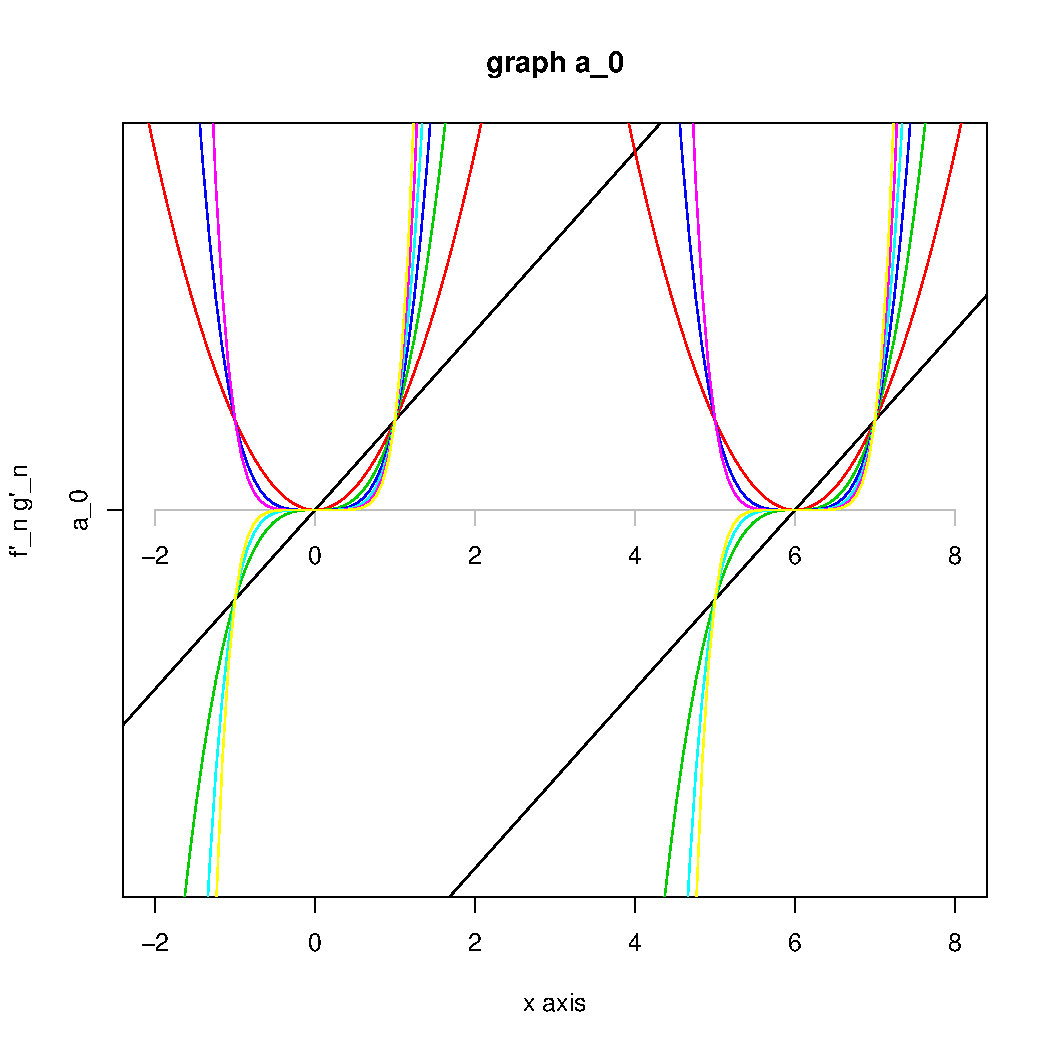
\includegraphics[scale=0.4]{graph2_R.pdf}
 \end{center}
\end{wrapfigure}
この関数$\hat{f}_n(x)$と$\hat{g}_n(x)$は
上の関数$f_n(x)$と$g_n(x)$に$a_0$を加えたものです。
加えた分だけ上下にずれます。
これらの関数は$a_0$に関係なく収束半径は$f_n$や$g_n$と同じです。
これらの関数の収束の仕方も同じですが、
$n\rightarrow\infty$の時の収束値は変わります。
図は$n=1,\dots,7$の時の$f^\prime_n$と$g^\prime_n$です。


$\hat{f}_n(x)$は区間$(-1,1)$内で収束します。
これは$a_0$の値が
$a_0\in(-1,1)$であっても、
$a_0\not\in(-1,1)$であっても収束します。
収束するかどうかは$a_0$の値に依存しません。
その為、収束を調べる場合は$a_0$の値を気にする必要はありません。



\end{document}
